\documentclass[aspectratio=169,xcolor=dvipsnames]{beamer}
\usetheme{Madrid}
\setbeamertemplate{navigation symbols}{}
\setbeamertemplate{footline}[frame number]

\usepackage{booktabs} % Allows the use of \toprule, \midrule and \bottomrule in tables
\usepackage[dutch]{babel}
\usepackage{amsmath,amssymb,amsfonts,textcomp, xfrac, bm} % wiskunde shizzel
\usepackage{graphicx} % foto's
%\setkeys{Gin}{draft}  % Skip missing images and render as placeholders
\usepackage{hyperref}
\usepackage{tikz} % Voor de tikz figuur hopelijk
\usetikzlibrary{angles,quotes, babel} % for pic (angle labels)
\usetikzlibrary{arrows.meta,decorations.markings,calc, decorations.pathmorphing, decorations.pathreplacing, positioning, shapes, shadings}
\usepackage{xcolor}

\hypersetup{
    colorlinks = false, 
    linkcolor = blue, 
    pdftitle = {Titel-van-pdf-bestand}
}

\newcommand{\blfootnote}[1]{%
  \begingroup
  \renewcommand{\thefootnote}{}%
  \footnotetext{#1}%
  \endgroup
}


\title{A Horseshoe Einstein Ring from Hubble}
\author{T. Cools}
\institute
{
    Bachelor Fysica en Sterrenkunde \\
    Faculteit Wetenschappen \\
    Universiteit Gent
}
\date{\today}

\begin{document}

\begin{frame}
  \titlepage
  \vfill
  \vspace{-0.4cm} % kleine correctie omhoog voor de logo's
  \begin{minipage}{0.45\textwidth}
        
\includegraphics[width=2cm]{../Figures-for-slides/logo_UGent_NL_RGB_2400_kleur-op-wit.png}
    \end{minipage}
    \hfill
    \begin{minipage}{0.45\textwidth}
        \raggedleft
        
\includegraphics[width=2cm]{../Figures-for-slides/icoon_UGent_WE_NL_RGB_2400_kleur-op-wit.png}
    \end{minipage}
\end{frame}


\begin{frame}{Introductie}

    %- Object: LRG 3-757 + gelensde achtergrondgalaxie
    %- Kernvraag: wat leren we over massa en centraal zwart gat?
    %- This interesting galaxy imaged by NASA’s Hubble Space Telescope is one of a group of galaxies called Luminous Red Galaxies. 
    % This blue horseshoe is a distant galaxy magnified and distorted by the strong gravitational pull of the massive foreground Luminous Red Galaxy. Called an Einstein Ring, this lensed galaxy required the exact alignment of the foreground and background galaxies, making this object’s nickname “the Cosmic Horseshoe” particularly apt. The Cosmic Horseshoe is one of the best examples of an Einstein Ring.
    
    \begin{figure}
        \centering
        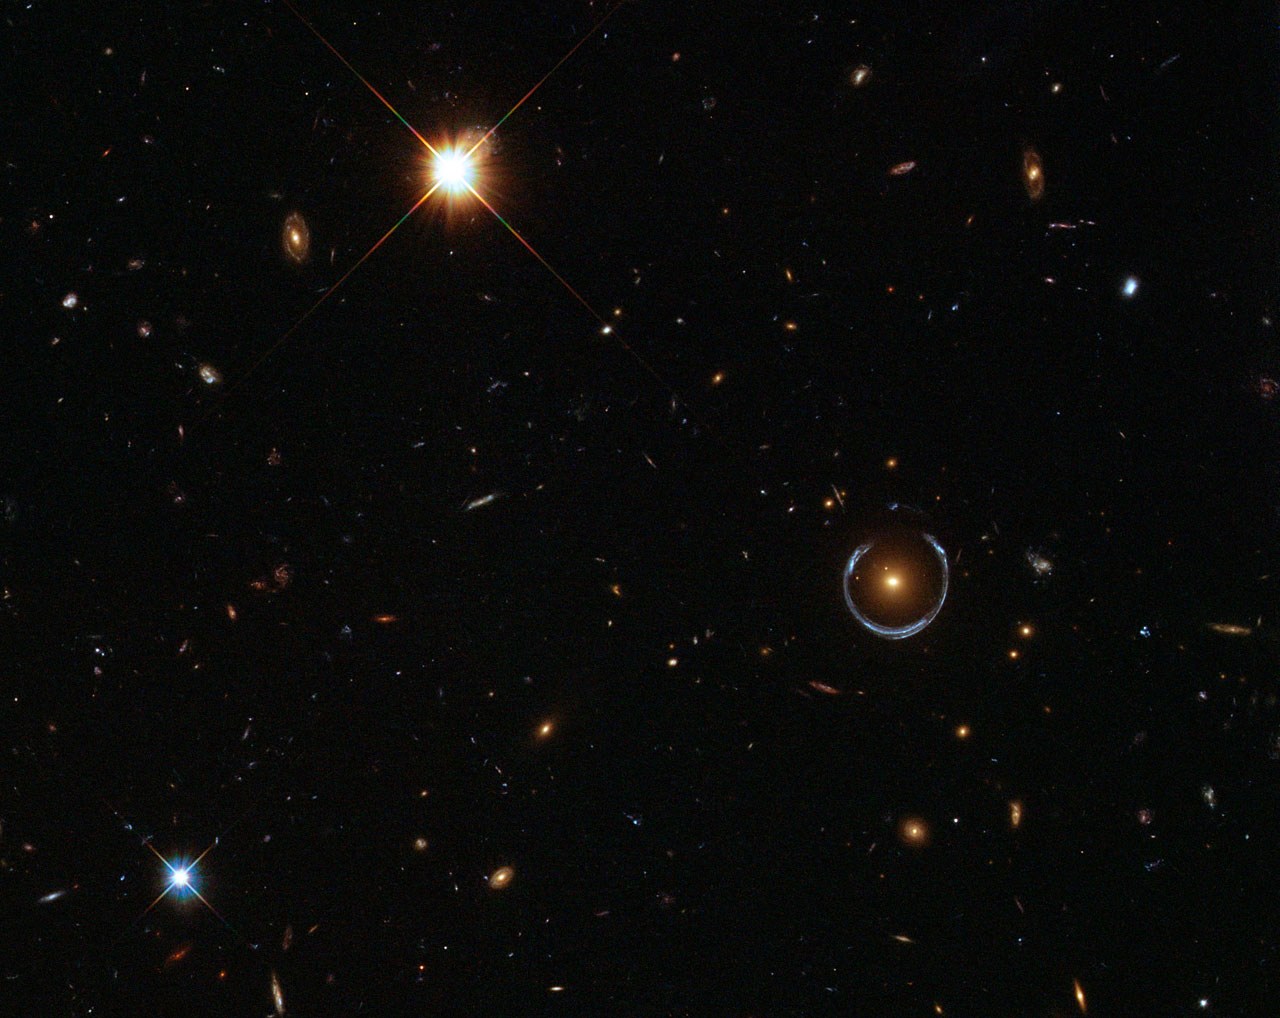
\includegraphics[width=0.55\linewidth]{../Figures-for-slides/potw1151a copy.jpg}
        \caption{A Horseshoe Einstein Ring from Hubble. \textit{\copyright \, ESA/Hubble \& NASA, 2011.}}
    \end{figure}

    
    % Example voor linken met cursus.
    %\blfootnote{\tiny Cursus §X.X — ...}
\end{frame}

\begin{frame}{Wat is een Einsteinring?}

%- Voorgrondmassa buigt licht van achtergrondbron
%- Bij bijna perfecte uitlijning ontstaat een ring
%- Ringstraal hangt samen met ingesloten massa

Gravitatielenzen ontstaan wanneer licht wordt afgebogen door de zwaartekracht van massieve objecten, zoals sterrenstelsels of clusters.
\begin{figure}
    \centering
    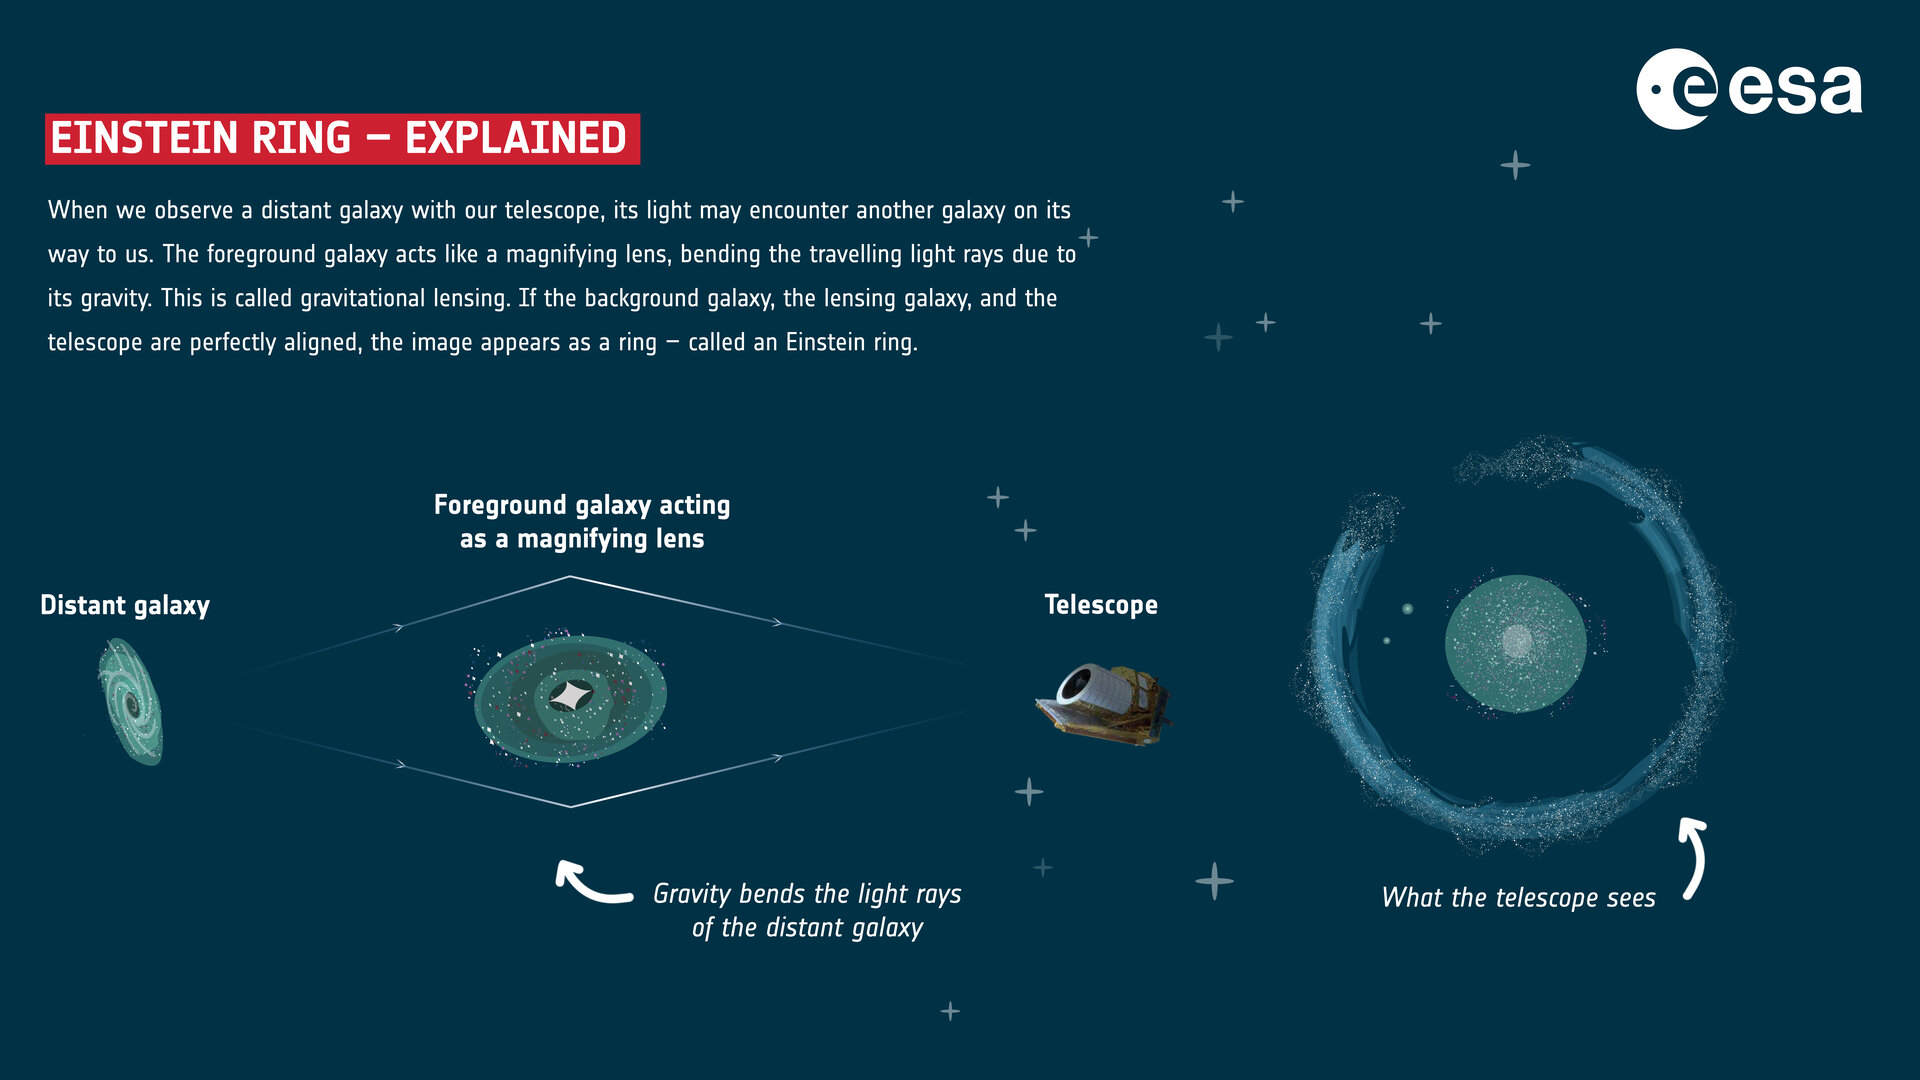
\includegraphics[width=0.5\linewidth]{../Figures-for-slides/Einstein_ring_explained_pillars.jpg}
    \caption{©ESA}
\end{figure}

De essentie van dit verschijnsel is dat donkere materie de dominante gravitationele component van clusters vormt.
\end{frame}

\begin{frame}{Het Cosmic Horseshoe systeem}
    \begin{columns}[T] % [T] zorgt ervoor dat beide kolommen aan de bovenkant uitlijnen
        
        % Linkerkolom voor de tekst
        \begin{column}{0.6\textwidth}
            \small
            % Ligt op 5 miljard lichtjaar verwijderd!!
            % Een van de meest massieve (ultramassive) black holes (UMBH) ooit waargenomen in het centrum.
            % Er wordt gedacht dat elke galaxie een (UMBH in het centrum heeft).
            % De UMBH in het hart van de Cosmic Horseshoe system wordt gedacht in de top 10 massiefste te zitten.

            % Astronomers first discovered the Cosmic Horseshoe in 2007 using data from the Sloan Digital Sky Survey. But this Hubble visible and infrared light image, taken with the Wide Field Camera 3, offers a much more detailed view of this fascinating object.
    

            Samengestelde lens met twee bronnen op verschillende roodverschuivingen.
            \vspace{0.2cm}

            Indien het achterliggende object vanuit het gezichtspunt van een waarnemer zeer precies is uitgelijnd met de lens, verschijnt er een ringvormige structuur, de Einsteinring.
            %Foto van de horseshoe (close up)

            \vspace{0.4cm}
            \begin{itemize}
                \item LRG 3-757 op de voorgrond met twee gelensde achtergrondgalaxies
                \item Hoe bepalen we de massa binnen een Einsteinring? 
                \item Is er een centraal zwart gat aanwezig?
                \item Kunnen we de gelensde sterrenstelsels reconstrueren?
            \end{itemize}

            \vspace{0.4cm}
             Probleem: tijdsdilatatie waarnemingen.
        \end{column}

        % Rechterkolom voor de figuur
        \begin{column}{0.38\textwidth}
            %\begin{figure}
                %\centering
                %\includegraphics[width=0.8\linewidth]{../Figures-for-slides/APOD-2025-FIG1.pdf}
                %\caption{\tiny HST/WFC3-kleurencomplex van de Cosmic Horseshoe, samengesteld met de F814W-, F606W- en F475W-filters. Het systeem bestaat uit de hoofdafbuiger ($z_l = 0.44$), de Einsteinring van de Cosmic Horseshoe ($z_{\text{s2}} = 2.381$), en de radiale boog met zijn tegenbeeld ($z_{s1} = 1.961$), die beide zijn uitgelicht. \copyright{C.~R. Melo-Carneiro et al. 2025. Published by Oxford University Press on behalf of Royal Astronomical Society.}}
            %\end{figure}
        \end{column}
        
    \end{columns}
\end{frame}

\begin{frame}{Luminous Red Galaxy}
    \begin{columns}[T] % [T] zorgt ervoor dat beide kolommen aan de bovenkant uitlijnen
        
        % Linkerkolom voor de tekst
        \begin{column}{0.6\textwidth}
            We houden rekening met 3 grote factoren en hun corresponderende roodverschuiving.
            
            \vspace{0.2cm}
            Lens: LRG in een groep van losse cluster in de quasar J1004+4112 met:
            
            \vspace{0.2cm}
            \begin{itemize}
                \item Roodverschuiving $z = 0.44$
                \item Snelheidsdispersie: $430 \pm 50$ km/s (2007) en $496 \pm 5$ km/s (2008)
            \end{itemize}

            \vspace{0.2cm}
            Voornaamste bron: Stervormend sterrenstelsel (type BX) met roodverschuiving tussen $z = 2.379-2.381$.
            % Misschien verklaring
            %It also gives us a tantalizing view of the early Universe: the blue galaxy’s redshift is approximately 2.4. This means we see it as it was about 3 billion years after the Big Bang. The universe is now 13.7 billion years old.

            \vspace{0.2cm}
            \textbf{Bijzonder:} Bijna het volledige lenseffect wordt veroorzaakt door de LRG alleen.

            \vspace{0.2cm}
        
            
        \end{column}

        % Rechterkolom voor de figuur
        \begin{column}{0.38\textwidth}
            %\begin{figure}
                %\centering
                %\includegraphics[width=0.8\linewidth]{../Figures-for-slides/APOD-2025-FIG1.pdf}
                %\caption{\tiny HST/WFC3-kleurencomplex van de Cosmic Horseshoe, samengesteld met de F814W-, F606W- en F475W-filters. Het systeem bestaat uit de hoofdafbuiger ($z_l = 0.44$), de Einsteinring van de Cosmic Horseshoe ($z_{\text{s2}} = 2.381$), en de radiale boog met zijn tegenbeeld ($z_{s1} = 1.961$), die beide zijn uitgelicht.\copyright{C.~R. Melo-Carneiro et al. 2025. Published by Oxford University Press on behalf of Royal Astronomical Society.}}
            %\end{figure}
        \end{column}
        
    \end{columns}
\end{frame}

\begin{frame}{Tracers}
    \begin{columns}[T] % [T] zorgt ervoor dat beide kolommen aan de bovenkant uitlijnen
        
        % Linkerkolom voor de tekst
        \begin{column}{0.4\textwidth}
            \small
            \begin{itemize}
                \item Rond spectroscopisch geïdentificeerde Quasars zoeken.
                \item Het doorzoeken van databases naar emissielijnen van objecten met hoge roodverschuiving in de spectra van vroeg-type sterrenstelsels met lage roodverschuiving.
                \item Het identificeren van blauwe, lichtzwakke begeleiders (faint companions) rond (LRG's) in de Sloan Digital Sky Survey (SDSS) cataloog.
                % De laatste is makkelijkst en snel om mee te experimenteren.
            \end{itemize}

            %\vspace{0.2cm}
        
            
        \end{column}

        % Rechterkolom voor de figuur
        \begin{column}{0.58\textwidth}
            \begin{figure}
                \centering
                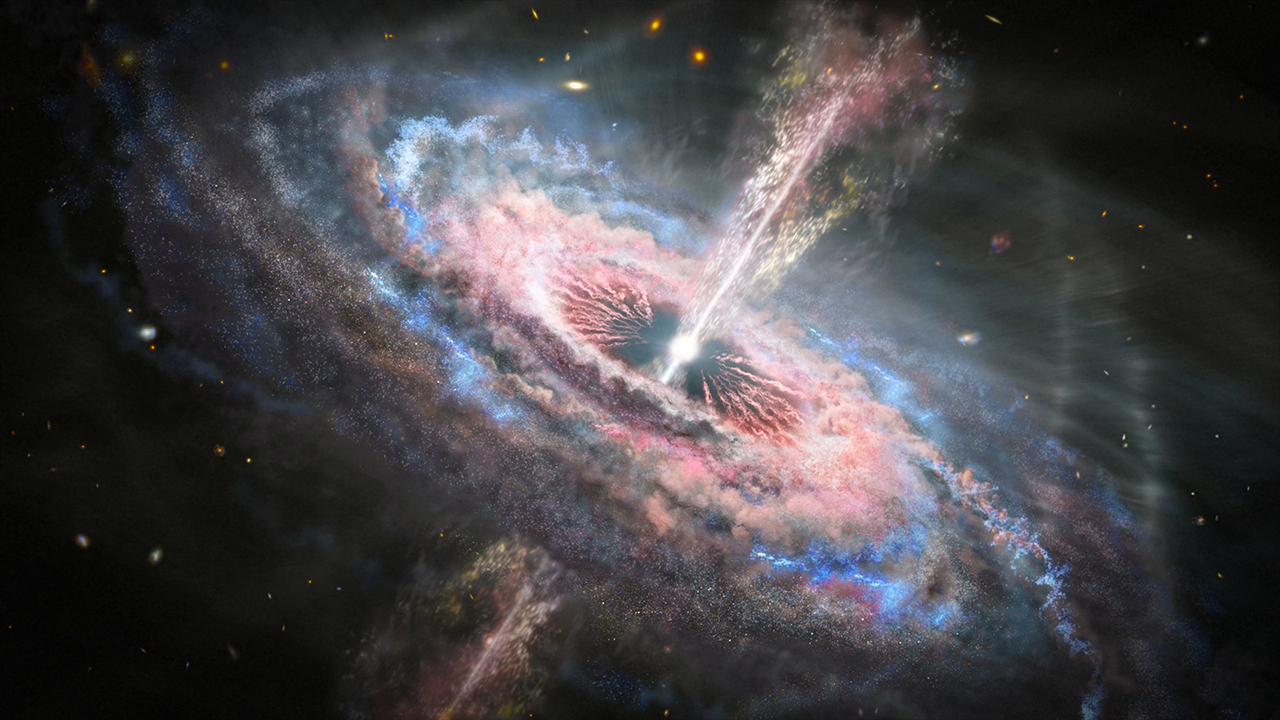
\includegraphics[width=\linewidth]{../Figures-for-slides/Quasar-Nasa.png}
                \caption{\tiny Artistieke impressie dat een ver sterrenstelsel met een actieve quasar in het centrum toont. Hubble ontdekte dat de stralingsdruk vanuit de nabijheid van het zwarte gat materie wegduwt uit het centrum van het stelsel met een fractie van de lichtsnelheid. Deze 'quasarwinden' stuwen jaarlijks honderden zonnemassa's aan materiaal naar buiten, de schijf van het sterrenstelsel in. Dit beïnvloedt het hele stelsel, doordat het materiaal zich als een sneeuwschuiver door het omringende gas en stof boort.\copyright{NASA, ESA and J. Olmsted (STScI)}}
            \end{figure}
        \end{column}
        
    \end{columns}
\end{frame}


\begin{frame}{Data \& instrumenten}
    \small
    Ontdekt in SDSS (2007), follow-up data:
  \begin{itemize}
    \item \small Isaac Newton Telescope (INT): Wide Field Camera 3, 600s in de i, g en u banden. (2007)
    \item \small HST (imaging), MUSE (kinematica). (C.~R. Melo-Carneiro et al. 2025.)
    %MUSE --> Multi Unit Spectroscopic Explorer
    %HST --> Hubble Space Telescope
    
    %\item Belangrijk: resolutie + kinematica reduceren systematiek.
  \end{itemize}


    \begin{columns}[t] % [t] zorgt dat de captions bovenaan uitlijnen als de tekst verschilt
        
        \begin{column}{0.48\textwidth}
            %\begin{figure}
                %\centering
                %\includegraphics[width=0.8\linewidth]{../Figures-for-slides/wfc3_inst-config.jpg}
                %\caption{\footnotesize Schematische voorstelling van WFC3. \copyright{NASA}}
            %\end{figure}
        \end{column}

        \begin{column}{0.48\textwidth}
            \begin{figure}
                \centering
                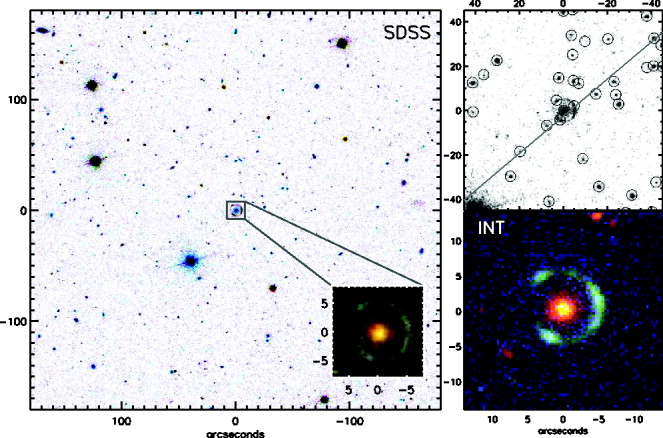
\includegraphics[width=0.8\linewidth]{../Figures-for-slides/FIG1-2007.jpeg}
                \caption{\footnotesize SDSS weergave rond de Cosmic Horseshoe. \copyright{V. Belokurov et al. 2007.}}
            \end{figure}
        \end{column}
        
    \end{columns}
  
  
\end{frame}


\begin{frame}{Gravitatielenzen I}
%Einstein schreef in 1936 dat we dit effect nooit zouden kunnen waarnemen, maar hij had daarbij enkel stellaire massa’s in gedachten. Het was onze oude bekende Fritz Zwicky die zich in 1937 realiseerde dat massieve clusters van sterrenstelsels we ́l in staat zijn om meerdere afbeeldingen van achterliggende sterrenstelsels te produceren.
    \small
    Algemene relativiteitstheorie:
    \[
    R_{\mu\nu} - \frac{1}{2}R\,g_{\mu\nu} + \Lambda g_{\mu\nu} = \frac{8\pi G}{c^4}T_{\mu\nu}
    \]
    Licht buigt af als gevolg van het gravitatie veld.
    %\begin{figure}
     %   \centering
      %  \includegraphics[width=0.6\linewidth]{../Figures-for-slides/grav-field-einstein.jpg}
       % \caption{Artistieke voorstelling van Gravity Probe B in een baan rond de aarde om ruimtetijd te meten, een vierdimensionale beschrijving van het heelal met hoogte, breedte, lengte en tijd.\copyright{NASA}}
    %\end{figure}
    \blfootnote{Zie General Relativity in de master }
\end{frame}

\begin{frame}{Gravitatielenzen II: Geometrie \& Vergelijkingen}
    \begin{columns}[T] % Uitlijnen op de bovenkant
        
        % Linkerkolom: De formules
        \begin{column}{0.55\textwidth}
            \small
            Algemene lensvergelijking: %(met meerdere oplossingen)
            \[
            \bm \beta = \bm \theta - \bm \alpha (\bm \theta)
            \]
            % 1 bron kan dus meerdere afbeeldingen produceren.
            Kritische oppervlaktedichtheid:
            \[
            \Sigma_{\mathrm{cr}} = \frac{c^2}{4\pi G}\,\frac{D_s}{D_lD_{ls}}
            \]% Bepaald of de lens sterk genoeg is om meervoudige afbeeldingen te produceren
            
            Einsteinstraal:
            \[
            \theta_E = \left({\frac{4GM(\theta_E)}{c^2}\frac{D_{ls}}{D_l D_s}}\right)^{\frac{1}{2}}
            \]
            
            \vspace{0.8cm}
            \blfootnote{Zie cursus: Structuur van het heelal}
        \end{column}

        % Rechterkolom: De figuur
        \begin{column}{0.42\textwidth}
            \begin{figure}
                \centering
                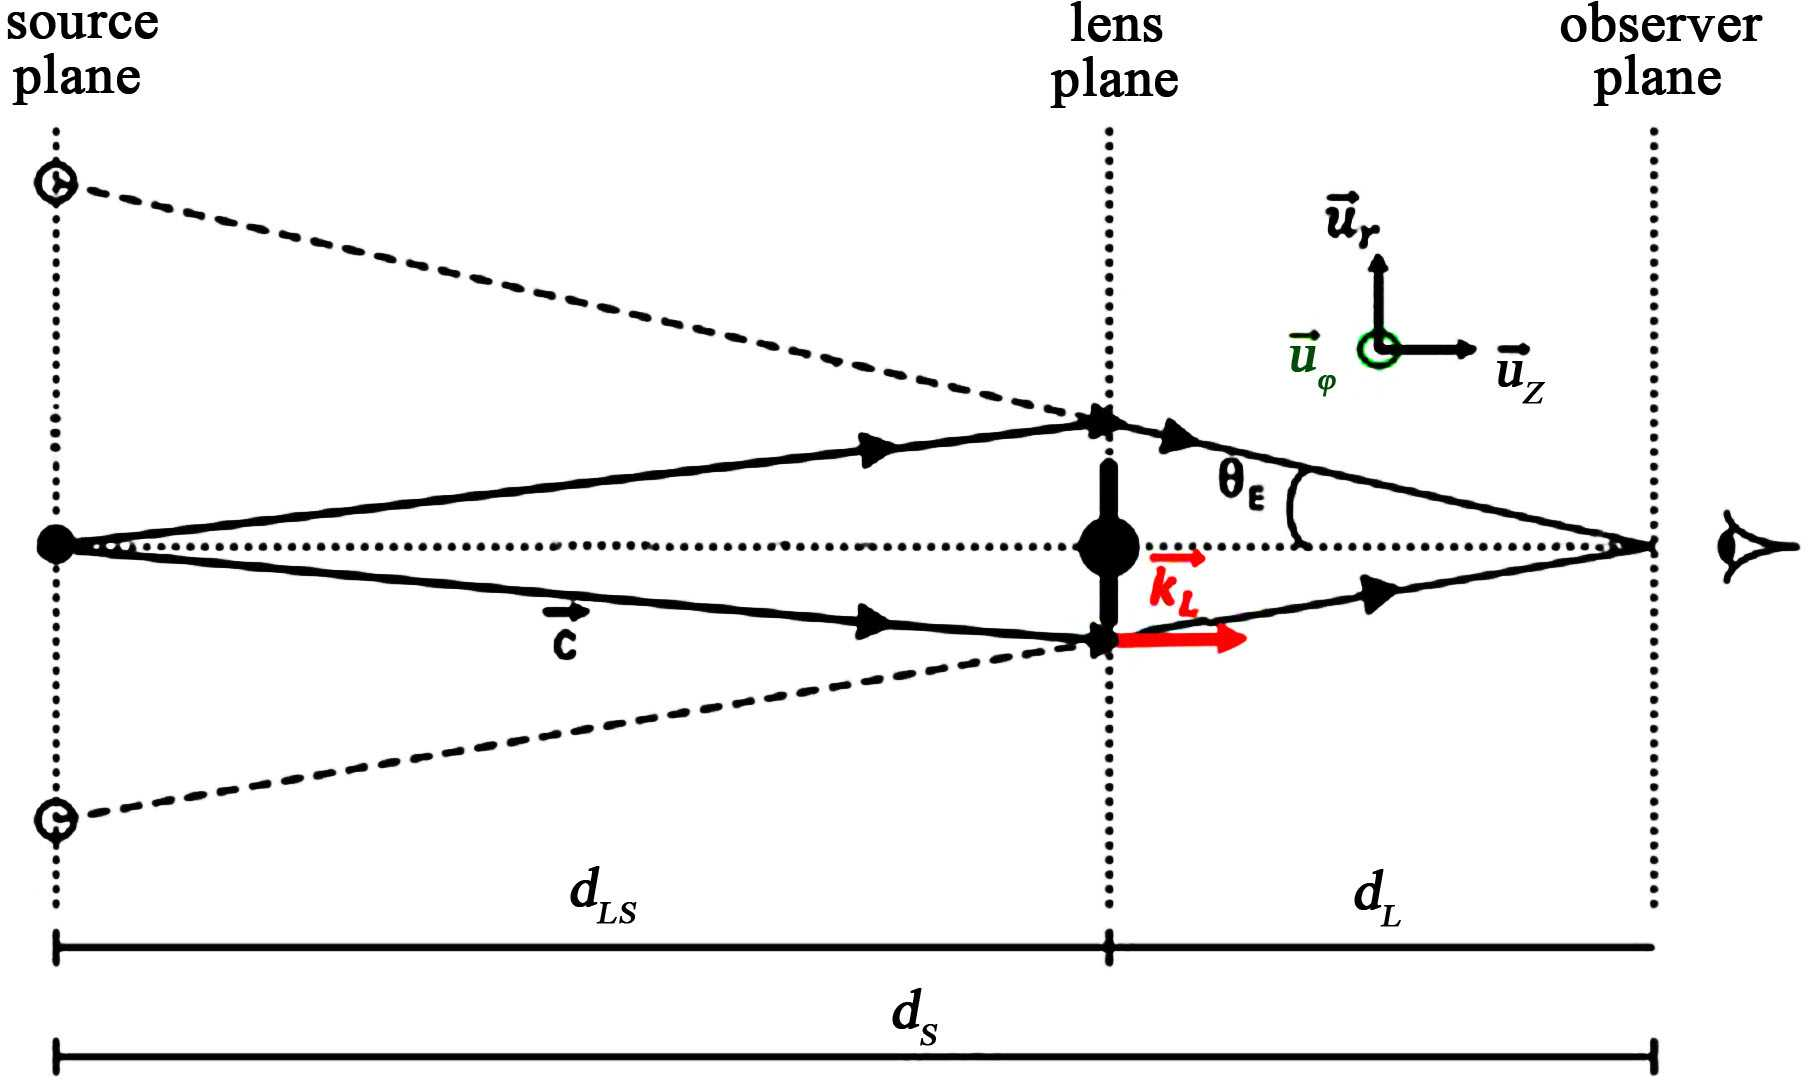
\includegraphics[width=\linewidth]{../Figures-for-slides/extra-paper-einsteinstraal.jpeg}
                \caption{\tiny Optische geometrie van een gravitationele lens, waarbij de Einsteinstraal $\theta_E$ de waargenomen hoek is als gevolg van het lenseffect op de schijnbare bron bij de waarnemer; $d_L$ is de hoekafstand tot de lens, $d_S$ is de hoekafstand tot de bron, en $d_{LS}$ is de hoekafstand tussen de lens en de bron; $\vec{k}_L$ is het gravitatieveld in de lens en $\vec{c}$ stelt de lichtstralen van de bron voor. \copyright{Le Corre, S. (2024) Gravitomagnetism and Gravitational Lens.}}
            \end{figure}
        \end{column}
        
    \end{columns}
\end{frame}


\begin{frame}{Modeleren}
    De beste modellen zijn te vinden door een evidence-functie \(\epsilon\) te maximaliseren:
    %om de verschillende modellen te rangschikken volgens de meest waarschijnlijke modellen.
    %Eventueel de functie
    \[ 
    -\ln \epsilon = \sum_j \left[\frac{\sum_i s_i f_{ij} - d_j}{\sigma_j}\right]^2
    + \ln\!\bigl[\det(\bm F + \lambda  \bm H)\bigr]
    - \ln\!\bigl[\det(\lambda \bm H)\bigr]
    + \lambda s^{T} \bm H s
    + \sum_j \ln\!\left(2\pi \sigma_j^2\right)
    \]
    %Somatie over j gaat over alle image pixels, en de somatie over i gaat over alle source pixels.
    Hierin is $f_{ij}$ de model-flux in pixel $j$, $d_j$ de gemeten flux met fout $\sigma_j$, $s_i$ de beste-fit bronvector, $\lambda$ de gewichtsfactoren en $\mathbf{F}, \mathbf{H}$ de vierkante regularisatiematrices.

    \vspace{0.2cm}
    De standaardfouten worden gegeven door de diagonale termen van de covariante matrix:
    \[
    \bm C = (\bm F + \lambda \bm H)^{-1}
    \]
    
\end{frame}




\begin{frame}{Dynamische modellering I}
    \small % Verkleint het standaard lettertype iets voor deze specifieke slide
    
    Jeans vergelijkingen:
    \vspace{-0.3cm} % Haalt de overtollige witruimte boven de formule weg
    \[
        \frac{\partial(\nu \overline{\upsilon_r^2})}{\partial r} + \frac{2 \nu \overline{\upsilon_r^2} - \nu \overline{\upsilon_\theta^2} - \nu \overline{\upsilon_\phi^2}}{r} = -\nu\frac{\partial \Phi}{\partial r} 
        \qquad \text{en} \qquad
        \frac{\partial (\nu\overline{\upsilon_\theta^2})}{\partial \theta} + \frac{\nu \overline{\upsilon_\theta^2 } - \nu \overline{\upsilon_\phi^2}}{\tan\theta} = - \nu\frac{\partial \Phi}{\partial \theta}
    \]
    
    \vspace{-0.1cm}
    Met \(\Phi\) de totale gravitatie potentiaal, \((\upsilon_r,\upsilon_\theta,\upsilon_\phi)\) de snelheden in sferische coördinaten en \(\nu\) de intrinsieke helderheidsdichtheid.
    
    %\vspace{-0.1cm}
    \begin{columns}[c]
        % Linkerkolom voor de laatste formule
        \begin{column}{0.45\textwidth}
            De stellaire anisotropie: 
            \[ 
            \beta = 1 - \frac{\overline{\upsilon_\theta^2}}{\overline{\upsilon_r^2}} = 1 - \frac{{\sigma_\theta}^2}{\sigma_r^2}
            \]
            De Jeans Anisotropic Modelling (JAM):

            \vspace{0.2cm}
            Benaderd de massadistributie als som van concentrische elliptische Gaussen.
            
            
            %gaat ervan uit dat de massadistributie geparametriseerd kan worden als een som van concentrische elliptische Gaussen. 
            
             

        \end{column}
    
        
        % Rechterkolom voor de afbeelding
        \begin{column}{0.5\textwidth}
            \begin{figure}
                \centering
                % Gebruik 'height' in plaats van 'width' om te forceren dat hij verticaal past
                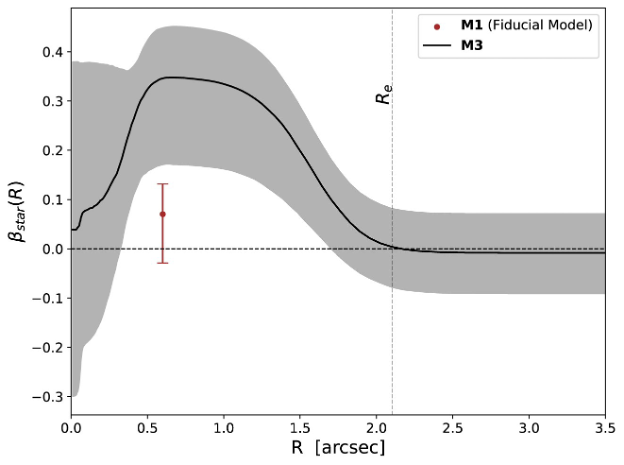
\includegraphics[width=0.75\linewidth]{../Figures-for-slides/Fig7-2025.png}
                \caption{\tiny Anisotropie profiel van model 3, met de gijze zone 1 \(\sigma\) afwijking.  \copyright{C.~R. Melo-Carneiro et al. 2025. Published by Oxford University Press on behalf of Royal Astronomical Society.}}
            \end{figure}
        \end{column}
    \end{columns}

    \vspace{-0.3cm}
    \blfootnote{Cursus: §9.3.1 Anisotropie in elliptische galaxieën}
\end{frame}

\begin{frame}{Dynamische modellering II}
    Randvoorwaarde: \(\nu \bar{\upsilon_r}^2= 0\) als \(r\to 0\).
    \[
    \upsilon_\phi^2 = (1 - \beta_{\text{star}}) \left[\overline{\upsilon_r^2} + \frac{\partial(\overline{\upsilon_r^2})}{\partial\theta} \tan\theta + \nu\frac{\partial\Phi}{\partial\theta} \tan\theta\right]
    \]
    
    
    \[
    \overline{\upsilon_r^2} = \int_r^{\infty} \left(\frac{r'}{r}\right)^{2\beta_{\text{star}}} \Psi(r', \theta') \, dr'
    \]
    
    Met
    \[
    \theta' = \arcsin\left[\left(\frac{r'}{r}\right)^{\beta_{\text{star}}-1} \sin\theta\right] 
    \]
    en
    \[
    \Psi(r,\theta) = \nu\left(\frac{\partial\Phi}{\partial r} - \frac{\tan\theta}{dr}\frac{\partial\Phi}{\partial\theta}\right)
    \]
    
\end{frame}

\begin{frame}{Resultaten: }
    \begin{figure}
        \centering
        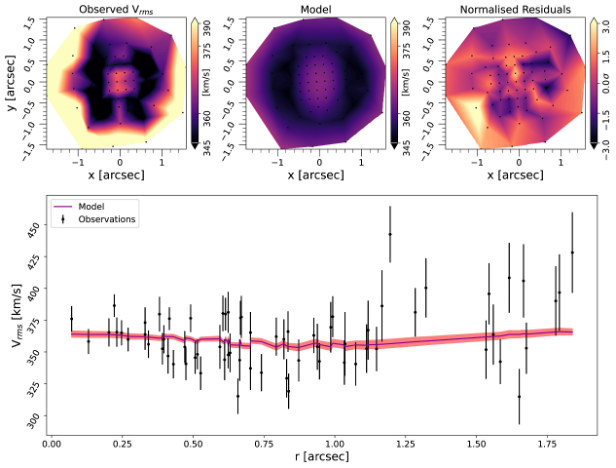
\includegraphics[width=0.5\linewidth]{../Figures-for-slides/Fig2-2025.png}
        \caption{\tiny Referentiemodel van de stellaire dynamica. De bovenste panelen tonen de geobserveerde $v_{\text{rms}}$ kinematische map (links), het mediaan kinematisch model (midden) en de genormaliseerde residuen (rechts). Het onderste paneel presenteert het radiale kinematische profiel (zwarte stippen) samen met het mediaan model en het bijbehorende $1\sigma$ betrouwbaarheidsinterval. De zwarte stippen in de bovenste panelen markeren de middelpunten van de Voronoi-bins. \copyright{C.~R. Melo-Carneiro et al. 2025. Published by Oxford University Press on behalf of Royal Astronomical Society.}}
    \end{figure}
\end{frame}


\begin{frame}{Het Massamodel I}
    We houden rekening met drie componenten:
    \begin{itemize}
        \item Stellaire massa component
        \item DM halo component
        \item Centraal geconcentreerde massa (SMBH)
    \end{itemize}

    \vspace{0.4cm}
    Elliptical Power-Law (EPL):
    \[
    \kappa(\xi) = \frac{(3-\gamma^{\text{lens}})}{1 + q^{\text{lens}}}\Big(\frac{\theta^{\text{lens}}_{\text{Ein}}}{\xi} \Big)^{\gamma^{\text{lens}}-1}
    \qquad
    \text{met}
    \qquad
    \xi = \sqrt{x^2+ \left(\frac{y}{q^{\text{lens}}}\right)^{2}}
    \]
    
    \vspace{0.2cm}
    \footnotesize
    $\gamma^{\text{lens}}$ is de massa-dichtheid helling, die tot een \textit{singular isothermal ellipsoid} (SIE) reduceert voor $\gamma^{\text{lens}}=2$.

    \blfootnote{Cursus: §2.4.1 Elliptische galaxieën} %De Isofoot (want stelsel is elliptisch, dus straal R wordt vervangen door \Xi).
\end{frame}

\begin{frame}{Het massa model II: Elliptische componenten}
    \begin{columns}[t] % [t] lijnt de kolommen aan de bovenkant uit
        
        % Linkerkolom: De Figuur
        \begin{column}{0.45\textwidth}
            %\begin{figure}
                %\centering
                %\includegraphics[width=0.8\linewidth]{../Figures-for-slides/APOD-2025-FIG1.pdf}
                %\caption{\tiny HST/WFC3-kleurencomplex van de Cosmic Horseshoe, samengesteld met de F814W-, F606W- en F475W-filters. \copyright{ C.~R. Melo-Carneiro et al. 2025.}}
            %\end{figure}
        \end{column}

        % Rechterkolom: De Tekst en Formules
        \begin{column}{0.55\textwidth}
            \small % Iets kleinere tekst past vaak beter bij twee kolommen
            
            Externe shears, geparametriseerd door $(\epsilon_1^{sh}, \epsilon_2^{sh})$.

            \vspace{0.5cm}
            De shear magnitude $\gamma^{sh}$ en shear hoek $\phi^{sh}$:
            \[
            \gamma^{sh} = \sqrt{{\epsilon_1^{sh}}^2 + {\epsilon_2^{sh}}^2}
            \]
            \[
            \tan(2\phi^{sh}) = \frac{\epsilon_2^{sh}}{\epsilon_1^{sh}}
            \]
            met
            \footnotesize
            \[
            \epsilon_1 = \frac{1-q^{\text{lens}}}{1+q^{\text{lens}}}\sin2\phi^{\text{lens}}  
            \qquad
            \text{en}
            \qquad 
            \epsilon_1 = \frac{1-q^{\text{lens}}}{1+q^{\text{lens}}}\cos2\phi^{\text{lens}}
            \]
        \end{column}
        
    \end{columns}
\end{frame}


\begin{frame}{Het massa model IV: DM halo}
    De donkere materie volgt een algemene Navarro-Frank-White (gNFW) profiel:
    \[  
    \rho(r) = \rho_s \left(\frac{r}{r_s}\right)^{-\gamma_{\mathrm{DM}}}
    \left(1 + \frac{r}{r_s}\right)^{\gamma_{\mathrm{DM}} - 3}
    \]
    met \(\rho_s\)  de karakteristieke dichtheid op straal \(r_s\) en \(\gamma_{DM}\) is de hellingsgraad van de DM-dichtheidsprofiel.
    \blfootnote{Cursus: §2.4.1 Elliptische galaxieën} %hellingsgraad
    \blfootnote{Cursus: §10.2 Donkere materie in elliptische galaxieën}
\end{frame}


\begin{frame}{Multi-Gaussian Expansion I}
    De MGE methode parametriseert de stellaire oppervlaktehelderheid als een som van concentrische elliptische Gaussen met dezelfde oriëntatie.
    \[
    I(x',y')=\sum_{j=1}^{N}\frac{L_j}{2\pi\sigma_j^{2}q'_j},\exp\left[-\frac{1}{2\sigma_j^{2}}\left(x'^2+\frac{y'^2}{(q'_j)^2}\right)\right]
    \]
    met \(I(x',y')\) de stellaire oppervlaktehelderheid,\(L_j\) de totale helderheid, \(N\) het totaal aantal Gaussen en dispersie \(\sigma_j\).

    \vspace{0.2cm}
    3-dimensionele helderheidsdichtheid \(\nu\) en bijbehorende massadichtheid verkregen door deprojectie met inclinatie \(i=90^\circ\).
    \blfootnote{Cursus: §2.3.2 Projectie in speciale geometriën}
    \blfootnote{Cursus: §9.1.3 Kinematische parameters}
\end{frame}

\begin{frame}{Multi-Gaussian Expansion II}
    \(\nu\) wordt omgezet naar stellaire massa door de massa-helderheid relatie \(\Upsilon_{\star}\).
    \[
    \rho(R,z)=\sum_{j=1}^{N}\frac{M_j}{(2\pi)^{3/2}\sigma_j^{3}q_j},\exp\left[-\frac{1}{2\sigma_j^{2}}\left(R^{2}+\frac{z^{2}}{q_j^{2}}\right)\right].
    \]
    met \(M_j = \Upsilon_{\star} L_j \)
    
    \vspace{0.2cm}
    De deprojectie as \(q_i\) wordt gegeven door:
    \[
    q_j^2 = \frac{q'^2_j-\cos^2 i}{\sin ^2 i}
    \]
    \blfootnote{Cursus: §2.3.2 Projectie in speciale geometriën}
    \blfootnote{Cursus: §9.2.3 Fysische betekenis van het Fundamentele Vlak}
    
\end{frame}

\begin{frame}{Resultaten I: Reconstructie}
    \begin{columns}%[t] % [t] zorgt dat de bovenkant van de kolommen uitlijnt
        
        \begin{column}{0.48\textwidth}
        \begin{itemize}
        \tiny
        \item V. Belokurov et al. (2007): \(\text{M}_{\text{Ein}}\sim 5.4\times10^{12}\text{M}_\odot\) 
        \item S. Dye et al. (2008): \(\text{M}_{\text{Ein}} =(5.02\pm0.09)\times10^{12}\text{M}_\odot\) (PL)
        %\item C. Alard et al. (2017): \(\text{M}_{\text{Ein}}=\)
        \item C.~R. Melo-Carneiro et al. (2025):
        \(\text{M}_{\text{Ein}} = (5.46\pm0.27)\times10^{12}\text{M}_\odot\) (EPL)\\
        en
        \( \log_{10}(\text{M}_\text{BH}/\text{M}_\odot ) = 10.56^{+0.07}_{-0.08} \pm (0.12)^{\text{sys}} \)
        \(\implies \text{M}_\text{BH} = 3.631^{+0.550}_{-0.625} \times 10^{10} \text{M}_\odot \)
    \end{itemize}
            \begin{figure}
                \centering
                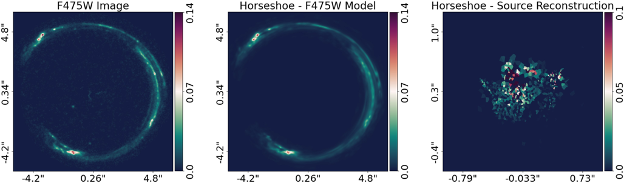
\includegraphics[width=\linewidth]{../Figures-for-slides/Fig3-2025.png}
                \caption{\tiny Fits aan de Cosmic Horseshoe in de F475W-filter. Van links naar rechts tonen de panelen het lens-gesubtraheerde beeld, het EPL-model met de hoogste waarschijnlijkheid, en de gereconstrueerde bron s2 bij $z = 2.381$. Alle beelden zijn uitgedrukt in eenheden van elektronen per seconde. \copyright{C.~R. Melo-Carneiro et al. 2025. Published by Oxford University Press on behalf of Royal Astronomical Society.}}
            \end{figure}
        \end{column}

        \begin{column}{0.48\textwidth}
            \begin{figure}
                \centering
                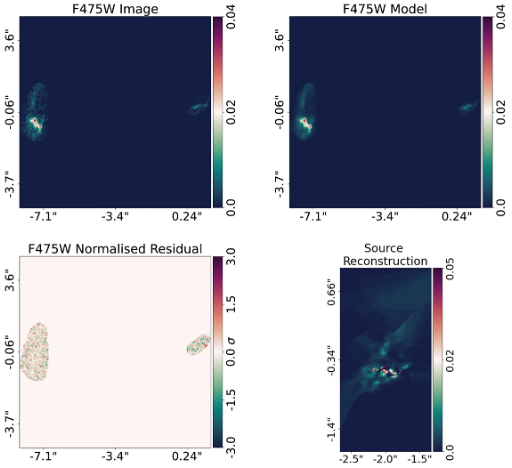
\includegraphics[width=0.75\linewidth]{../Figures-for-slides/Fig5-2025.png}
                \caption{\tiny Meest waarschijnlijke lensmodel onder de referentieconfiguratie. De panelen tonen, van linksboven naar rechtsonder, de geobserveerde afbeelding, het model van de gelensde bron, de genormaliseerde residuen en de reconstructie van de bron. Alle afbeeldingen zijn weergegeven in eenheden van elektronen per seconde. \copyright{C.~R. Melo-Carneiro et al. 2025. Published by Oxford University Press on behalf of Royal Astronomical Society.}}
            \end{figure}
        \end{column}
        
    \end{columns}
\end{frame}



\begin{frame}[shrink=10]{Centraal SMBH noodzakelijk?}
% Uitleg over de supermassive black hole
Als de evidence wordt toegepast op de modellen met en zonder een zwart gat:
\begin{table}[htbp]
\caption{Resultaten voor 15 verschillende modellen. \copyright{C.~R. Melo-Carneiro et al. (2025)}}
\centering
\tiny
\renewcommand{\arraystretch}{1.15}
\resizebox{\textwidth}{!}{%
\begin{tabular}{llcccc}
\toprule
Model ID & Mass model & $\log_{10}(M_{\mathrm{BH}}/M_\odot)$ & $\Delta \ln Z$ & Section & $N_{\mathrm{par}}$ \\
\midrule
M1  & $\Upsilon_\star + \mathrm{ell.}\ \mathrm{NFW}\ (r_s=10R_e) + \beta_\star + \mathrm{BH}$
    & $10.56^{+0.07}_{-0.08}$ & $0.00$  & 4.1     & 8  \\
M2  & $\Upsilon_\star + \mathrm{ell.}\ \mathrm{gNFW}\ (r_s=10R_e) + \beta_\star + \mathrm{BH}$
    & $10.57^{+0.07}_{-0.09}$ & $-0.53$ & 4.2.1.1 & 9  \\
M3  & ${}^{3}\Upsilon_\star + \mathrm{ell.}\ \mathrm{NFW}\ (r_s=10R_e) + {}^{3}\beta_\star + \mathrm{BH}$
    & $10.45^{+0.11}_{-0.14}$ & $-3.48$ & 4.2.1.2 & 10 \\
M4  & ${}^{3}\Upsilon_\star + \mathrm{ell.}\ \mathrm{NFW}\ (r_s=10R_e) + \beta_\star + \mathrm{BH}$
    & $10.53^{+0.10}_{-0.11}$ & $2.01$  & 4.2.1.3 & 10 \\
M5  & $\Upsilon_\star + \mathrm{ell.}\ \mathrm{NFW} + \beta_\star + \mathrm{BH}$
    & $10.56^{+0.08}_{-0.08}$ & $-0.38$ & 4.2.1.4 & 9  \\
M6  & $\Upsilon_\star + \mathrm{ell.}\ \mathrm{NFW}\ (r_s=10R_e) + \beta_\star + \mathrm{BH}$\\
    & \hspace{1.5em}\emph{w/ cyl. velocity ellipsoids}
    & $10.55^{+0.08}_{-0.09}$ & $-0.36$ & 4.2.1.5 & 8  \\
M7  & $\Upsilon_\star + \mathrm{ell.}\ \mathrm{NFW}\ (r_s=10R_e) + \beta_\star + \mathrm{BH}$\\
    & \hspace{1.5em}\emph{w/ Delaunay pixelisation}
    & $10.55^{+0.08}_{-0.08}$ & $-2.27$ & 4.2.1.5 & 8  \\
M8  & $\Upsilon_\star + \mathrm{ell.}\ \mathrm{NFW}\ (r_s=10R_e) + \beta_\star + \mathrm{BH}$\\
    & \hspace{1.5em}\emph{w/o Horseshoe}
    & $10.51^{+0.07}_{-0.09}$ & $0.38$  & 4.2.1.5 & 8  \\
M9  & ${}^{3}\Upsilon_\star + \mathrm{ell.}\ \mathrm{gNFW}\ (r_s=10R_e) + {}^{3}\beta_\star + \mathrm{BH}$
    & $10.50^{+0.10}_{-0.32}$ & $8.29$  & 4.2.2   & 13 \\
M10 & $\mathrm{Gaussian}\ \Upsilon_\star + \mathrm{sph.}\ \mathrm{NFW}\ (r_s=10R_e) + {}^{8}\beta_\star + \mathrm{BH}$
    & $10.55^{+0.10}_{-0.07}$ & $1.17$  & 4.2.2   & 16 \\
M11 & ${}^{3}\Upsilon_\star + \mathrm{ell.}\ \mathrm{gNFW}\ \mathrm{w/}\ \mathrm{main}\ c(M,z) + {}^{3}\beta_\star + \mathrm{BH}$
    & $10.15^{+0.17}_{-0.30}$ & $2.92$  & 4.2.2   & 13 \\
M12 & ${}^{3}\Upsilon_\star + \mathrm{ell.}\ \mathrm{gNFW}\ \mathrm{w/}\ 1\sigma\ \mathrm{below}\ c(M,z) + {}^{3}\beta_\star + \mathrm{BH}$
    & $10.33^{+0.07}_{-0.13}$ & $10.73$ & 4.2.2   & 13 \\
M13 & ${}^{3}\Upsilon_\star + \mathrm{ell.}\ \mathrm{gNFW}\ \mathrm{w/}\ 1\sigma\ \mathrm{above}\ c(M,z) + {}^{3}\beta_\star + \mathrm{BH}$
    & $10.59^{+0.04}_{-0.10}$ & $11.48$ & 4.2.2   & 13 \\
M14 & $\Upsilon_\star + \mathrm{ell.}\ \mathrm{NFW}\ (r_s=10R_e) + \beta_\star$
    & $-$ & $16.31$ & 4.3 & 7 \\
M15 & ${}^{3}\Upsilon_\star + \mathrm{ell.}\ \mathrm{NFW}\ (r_s=10R_e) + \beta_\star$
    & $-$ & $11.17$ & 4.3 & 9 \\
\bottomrule
\end{tabular}%
}
\end{table}

\end{frame}

\begin{frame}{Star Formation Rate}
Het verschil tussen de Ly \(\alpha\) emissie en de interstellaire absorbtie roodverschuiving wordt typisch gevonden bij sterrenstelsels met een hoge SFR. De Ly \(\alpha\) lijn correspondeert normaal met 1216Å wordt hier verschoven naar \(\approx \)4100Å.
    \begin{figure}
        \centering
        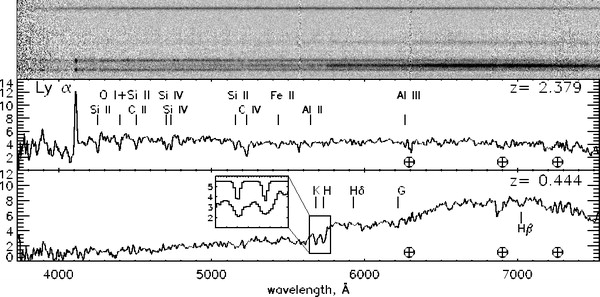
\includegraphics[width=0.5\linewidth]{../Figures-for-slides/FIG4-2007.jpeg}
        \caption{\footnotesize Het bovenste spectrum toont dat de bron een stervormend sterrenstelsel is bij een roodverschuiving van \(z = 2.379\). \(\bigoplus\) is de absorptie door de aardatmosfeer. \copyright{V. Belokurov et al. 2007.} }
    \end{figure}
    % Eventuele verklaring:
    % It also gives us a tantalizing view of the early Universe: the blue galaxy’s redshift is approximately 2.4. This means we see it as it was about 3 billion years after the Big Bang. The universe is now 13.7 billion years old.
    \blfootnote{Cursus: §3.2.3 Warm geïoniseerd gas}
    \blfootnote{Cursus: H6 Stervorming}
\end{frame}

\begin{frame}{Tijddilatatie}

\[
\Delta t = \frac{2D_d}{c}\theta_E^2
\]

%\begin{figure}
    %\centering
    %\includegraphics[width=0.5\linewidth]{../Figures-for-slides/fg5.h.jpg}
    %\caption{\tiny Contouren van het Fermat-tijddilatatie-oppervlak voor twee mogelijke lensmodellen van de Cosmic Horseshoe, samen met de locaties van de stationaire punten die de voorspelde beeldposities markeren. De kritieke curve van het lensmodel, die ook een contour van constante convergentie is, wordt in rood weergegeven, samen met de waargenomen beeldlocaties. \copyright{V. Belokurov et al. 2007.}}
%\end{figure}

    
\end{frame}

\begin{frame}{Resultaten II: \(\text{M}_{\text{BH}}-\sigma_e\) relatie}
    \begin{figure}
        \centering
        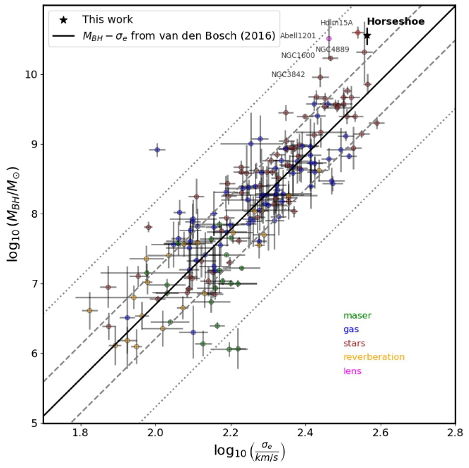
\includegraphics[width=0.42\linewidth]{../Figures-for-slides/fig10-2025.png}
        \caption{\tiny Relatie tussen $M_\text{BH}$-massa en de effectieve snelheidsdispersie van de gastheer. De zwarte volle lijn stelt de relatie van den Bosch (2016) voor, met de gestippelde en puntgestippelde lijnen die respectievelijk de $1\sigma$- en $3\sigma$-verstrooiing tonen. Cosmic Horseshoe, bij $z_l = 0.44$, vertegenwoordigt een van de meest massieve SMBHs die zijn gemeten en is een ongeveer $1.5\sigma$-uitschieter van de hoofdrelatie van $M_\text{BH}\!-\!\sigma_e$. De SMBH-massasamenvatting is afkomstig van den Bosch (2016).\copyright{C.~R. Melo-Carneiro et al. 2025. Published by Oxford University Press on behalf of Royal Astronomical Society.}}
        
    \end{figure}
\blfootnote{Cursus: §9.2.1 De Faber-Jackson relatie}        
\end{frame}

\begin{frame}{Wat weten we nog niet?}
    % De drie mogelijkheden van paper 2025 Sectie discussies
    \begin{itemize}
        \item De Cosmic Horseshoe behoord mogelijks een fossielgroep
        \item UMBH's zouden overblijfselen kunnen zijn van extreem lichtsterke quasars actieve galactische kernen waarin superzware zwarte gaten in het vroege heelal in korte tijd sterk zijn gegroeid door snelle accretie.
        \item Als de SMBH in de Cosmic Horseshoe inderdaad een UMBH is, dan zou dit kunnen wijzen op een scenario waarin de groei van het zwarte gat sneller is verlopen dan die van de gastheer, wat suggereert dat SMBH-groei niet altijd nauw verbonden is met de evolutie van het gaststelsel.
        \item De ontdekking van een UMBH in de Cosmic Horseshoe kan ook implicaties hebben voor ons begrip van de co-evolutie van SMBH's en hun gaststelsels, en kan wijzen op de noodzaak om bestaande modellen van deze co-evolutie te herzien.
        \item De aanwezigheid van een UMBH in de Cosmic Horseshoe kan ook gevolgen hebben voor onze kennis van de rol van SMBH's in het vroege heelal, en kan ons helpen om beter te begrijpen hoe deze objecten zich hebben gevormd en geëvolueerd in de context van de kosmische geschiedenis.
        \item 

    \end{itemize}
\end{frame}

\begin{frame}{Eigen onderzoeksvoorstel}
    Wat zou beter kunnen?
    \begin{itemize}
        \item Betere waarnemingen, er is nood aan extra data
        \item Data over Einsteinringen is beperkt op dit moment
        
    \end{itemize}

    Mogelijke oplossingen:
    \begin{itemize}
        \item Euclid mission om meer lenzen te ontdekken in de nabijee 5 jaar.
        \item De Extremely Large Telescope (ELT) zal de mogelijkheid om de dynamica te bestuderen vergroten. 
    \end{itemize}
    Eigen voorstellen:
    \begin{itemize}
        \item Tijddilatatie van het systeem onderzoeken 
        \item Hoge-resolutie spectroscopie + diepere imaging, zal voor een kleinere fout zorgen dat we de beste modellen kunnen aantonen wat meer zekerheid geeft.
        \item Meer lenzen bestuderen, zodat we een grotere steekproef hebben van SMBH's in Einsteinringen.
        \item Het gedetailleerde modelering zal de studie naar de interactie tussen baryonen en donkere materie in zeer massieve sterrenstelsels mogelijk maken.
    \end{itemize}

    
\end{frame}


\begin{frame}{Bibliografie}
  \begin{thebibliography}{9}

    \bibitem{belokurov2007}
    V. Belokurov et al. 2007.
    \textit{The Cosmic Horseshoe: Discovery of an Einstein Ring around a Giant Luminous Red Galaxy.}
    ApJ, 671(1), L9–L12.
    \href{https://doi.org/10.1086/524948}{doi:10.1086/524948}

    \bibitem{dye2008}
    S. Dye et al. 2008.
    \textit{Models of the Cosmic Horseshoe gravitational lens J10044112.}
    MNRAS.
    \href{https://doi.org/10.1111/j.1365-2966.2008.13401.x}{doi:10.1111/j.1365-2966.2008.13401.x}

    

    \bibitem{LeCorre2024}
    Le Corre, S. 2024. Gravitomagnetism and Gravitational Lens. Open Access Library Journal, 11, 1-11. \href{https://www.scirp.org/journal/paperinformation?paperid=138088}{doi: 10.4236/oalib.1112628.}

    \bibitem{melocarneiro2025}
    C.~R. Melo-Carneiro et al. 2025.
    \textit{Unveiling a 36 billion solar mass black hole at the centre of the Cosmic Horseshoe.}
    MNRAS, 541(4), 2853–2871.
    \href{https://doi.org/10.1093/mnras/staf1036}{doi:10.1093/mnras/staf1036}

    

    
  \end{thebibliography}
\end{frame}

\end{document}
